\documentclass{standalone}

\usepackage{unicode-math} % Euler virtual math fonts.
\usepackage{tikz}

\usetikzlibrary{external}
\usetikzlibrary{arrows.meta} % Advanced arrow tip library.
\usetikzlibrary{calc} % Coordinate calculations.

\definecolor{wwqqcc}{rgb}{0.4, 0, 0.8}
\definecolor{qqzzqq}{rgb}{0, 0.6, 0}
\definecolor{ffwwqq}{rgb}{1, 0.4, 0}

\setmathfont{Euler Math}

\tikzexternalize % activate externalization
\tikzsetnextfilename{mouldoverall.pdf}

\begin{document}
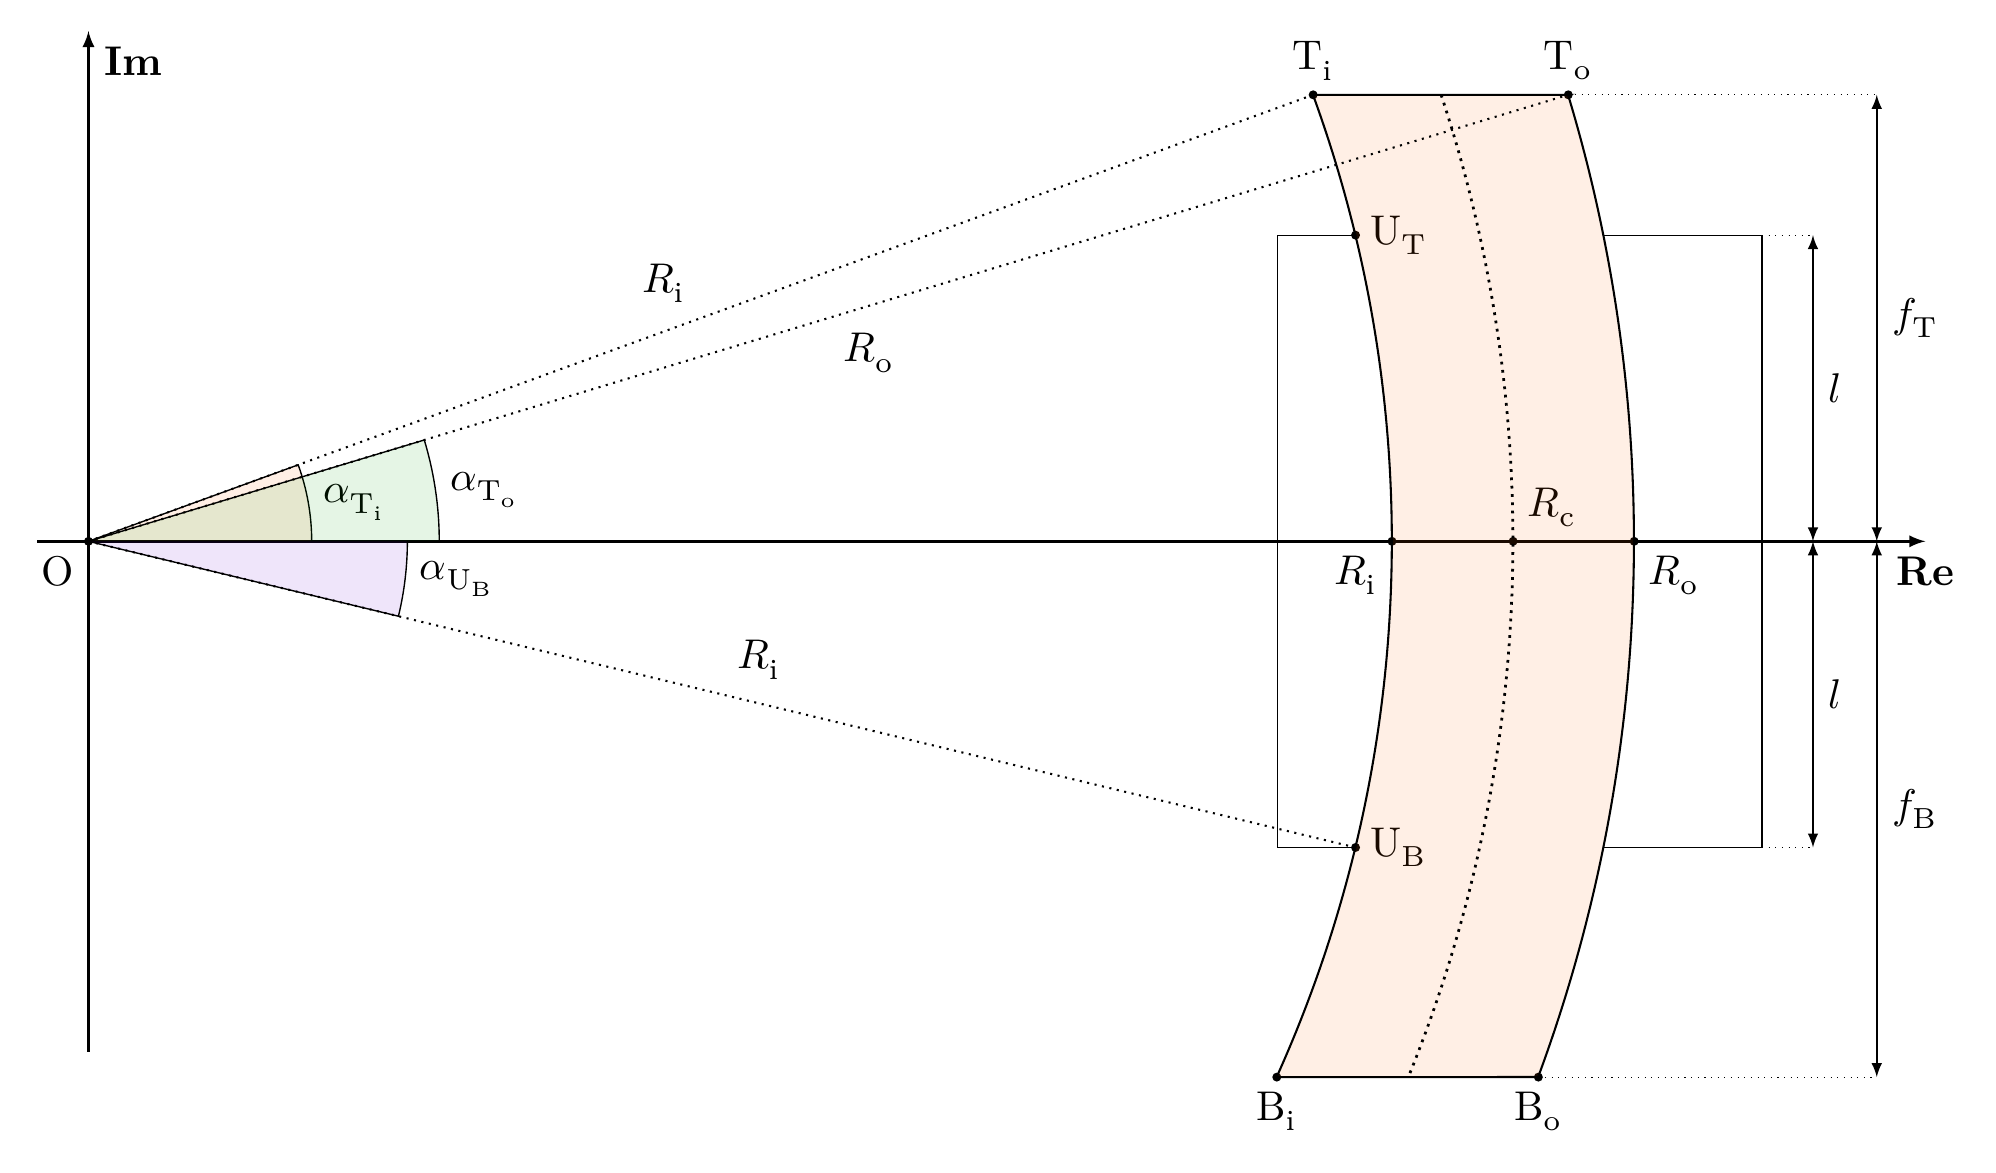
\begin{tikzpicture}[scale=1.62, every node/.style={scale=1.5}]
% 値の計算
\pgfmathsetmacro{\Ax}{9.6} %A:T_iのx座標
\pgfmathsetmacro{\Ay}{3.5} %A:T_iのy座標
\pgfmathsetmacro{\Bx}{2.0+(\Ax)} %B:T_oのx座標
\pgfmathsetmacro{\Cy}{-4.2}                  %C:B_iのy座標
\pgfmathsetmacro{\Ri}{sqrt((\Ax)^2+(\Ay)^2)} %R_iの長さ
\pgfmathsetmacro{\Cx}{sqrt((\Ri)^2-(\Cy)^2)} %C:B_iのx座標
\pgfmathsetmacro{\Ro}{sqrt((\Bx)^2+(\Ay)^2)} %R_oの長さ
\pgfmathsetmacro{\Dx}{sqrt((\Ro)^2-(\Cy)^2)} %D:B_oのx座標
\pgfmathsetmacro{\Rc}{(\Ri+\Ro)/2}           %R_cの長さ
\pgfmathsetmacro{\Ex}{sqrt((\Rc)^2-(\Ay)^2)} %E:湾曲中心線トップ端のx座標
\pgfmathsetmacro{\Fx}{sqrt((\Rc)^2-(\Cy)^2)} %F:湾曲中心線ボトム端のx座標
\pgfmathsetmacro{\Ub}{2.4}                   %Ub:受板-モールド接点のy座標
\pgfmathsetmacro{\Ux}{sqrt((\Ri)^2-(\Ub)^2)} %Ux:受板-モールド接点のx座標
\pgfmathsetmacro{\Uxo}{sqrt((\Ro)^2-(\Ub)^2)} %Ux:受板-モールド接点のx座標
\pgfmathsetmacro{\Hx}{1+(\Ri)} %H:テーブルの中心
\pgfmathsetmacro{\Ix}{1.90} %I:テーブルx方向の長さの半分
% 座標系を描画
\draw[-latex, line width=1pt] (-0.4, 0) -- (14.4, 0) node[below] {\textbf{Re}};
\draw[-latex, line width=1pt] (0, -4) -- (0, 4) node[below right] {\textbf{Im}};
% 座標を定義
\coordinate (O) at (  0, 0); % 原点
\coordinate (A) at (\Ax, \Ay); %
\coordinate (B) at (\Bx, \Ay);
\coordinate (C) at (\Cx, \Cy);
\coordinate (D) at (\Dx, \Cy);
\coordinate (E) at (\Ex, \Ay);
\coordinate (F) at (\Fx, \Cy);
\coordinate (Rc) at (\Rc, 0);
\coordinate (Ri) at (\Ri, 0);
\coordinate (Ro) at (\Ro, 0);
\coordinate (Ut) at (\Ux, \Ub);
\coordinate (Ub) at (\Ux, -\Ub);
\coordinate (Uto) at (\Uxo, \Ub);
\coordinate (Ubo) at (\Uxo, -\Ub);
\coordinate (Tal) at (\Hx-\Ix, \Ub);
\coordinate (Tbl) at (\Hx-\Ix, -\Ub);
\coordinate (Tar) at (\Hx+\Ix, \Ub);
\coordinate (Tbr) at (\Hx+\Ix, -\Ub);
\coordinate (Lt) at (\Hx+\Ix+0.4, \Ub);
\coordinate (Lb) at (\Hx+\Ix+0.4, -\Ub);
\coordinate (Lc) at (\Hx+\Ix+0.4, 0);
\coordinate (Fc) at (\Hx+\Ix+0.9, 0);
\coordinate (Ft) at (\Hx+\Ix+0.9, \Ay);
\coordinate (Fb) at (\Hx+\Ix+0.9, \Cy);
% 点を描画
\fill (O) circle (1pt);
\fill (A) circle (1pt);
\fill (B) circle (1pt);
\fill (C) circle (1pt);
\fill (D) circle (1pt);
%\fill (E) circle (1pt);
\fill (Rc) circle (1pt);
\fill (Ro) circle (1pt);
\fill (Ri) circle (1pt);
\fill (Ut) circle (1pt);
\fill (Ub) circle (1pt);
% 点にラベルを付ける
\node at (O) [below left] {O};
\node at (A) [above] {T$_\mathrm i$};
\node at (B) [above] {T$_\mathrm o$};
\node at (C) [below] {B$_\mathrm i$};
\node at (D) [below] {B$_\mathrm o$};
\node at (Rc) [above right] {$R_\mathrm c$};
\node at (Ro) [below right] {$R_\mathrm o$};
\node at (Ri) [below left] {$R_\mathrm i$};
\node at (Ut) [right] {U$_\mathrm T$};
\node at (Ub) [right] {U$_\mathrm B$};
% モールド外形
\draw[line width=0.75pt, fill=ffwwqq, fill opacity=0.1]
  let \p1=(A), \p2=(C), \p3=(B), \p4=(D), \n1={atan2(\y1,\x1)}, \n2={atan2(\y2,\x2)}, \n3={atan2(\y3,\x3)}, \n4={atan2(\y4,\x4)}
    in (A) -- (B) -- (\n3:\Ro) arc (\n3:\n4:\Ro) -- (C) -- (\n2:\Ri) arc (\n2:\n1:\Ri) -- cycle;
% モールド中心線
\draw[dotted, line width=1pt] let \p1=(E), \p2=(F), \n1={atan2(\y1,\x1)}, \n2={atan2(\y2,\x2)}
  in (\n1:\Rc) arc (\n1:\n2:\Rc);
% テーブル
\draw (Ut) -- (Tal) -- (Tbl) -- (Ub);
\draw (Uto) -- (Tar) -- (Tbr) -- (Ubo);
\draw[dotted] (Tar) -- (Lt);
\draw[dotted] (Tbr) -- (Lb);
\draw[dotted] (Tar) -- (Lt);
\draw[latex-latex, line width=0.75pt] (Lc) -- (Lt) node[midway, right] {$l$};
\draw[latex-latex, line width=0.75pt] (Lc) -- (Lb) node[midway, right] {$l$};
% 振分け
\draw[dotted] (B) -- (Ft);
\draw[dotted] (D) -- (Fb);
\draw[latex-latex, line width=0.75pt] (Fc) -- (Ft) node[midway, right] {$f_\mathrm T$};
\draw[latex-latex, line width=0.75pt] (Fc) -- (Fb) node[midway, right] {$f_\mathrm B$};
% 半径
\draw[dotted, line width=0.75pt] (O) -- (A) node[midway, above left] {$R_\mathrm i$} ;
\draw[dotted, line width=0.75pt] (O) -- (B) node[midway, below right] {$R_\mathrm o$} ;
\draw[dotted, line width=0.75pt] (O) -- (Ub) node[midway, above right] {$R_\mathrm i$} ;
% 角度
\draw[line width=0.5pt, fill=ffwwqq, fill opacity=0.1]
  let \p1=(Ri), \p2=(A), \n1={atan2(\y1,\x1)}, \n2={atan2(\y2,\x2)}
   in (\n1:1.75) arc (\n1:\n2:1.75) node[midway, right, opacity=1] {$\alpha_{\mathrm T_\mathrm i}$} -- (O);
\draw[line width=0.5pt, fill=qqzzqq, fill opacity=0.1]
  let \p1=(Ro), \p2=(B), \n1={atan2(\y1,\x1)}, \n2={atan2(\y2,\x2)}
  in (\n1:2.75) arc (\n1:\n2:2.75) node[midway, right, opacity=1] {$\alpha_{\mathrm T_\mathrm o}$} -- (O) -- cycle ;
\draw[line width=0.5pt, fill=wwqqcc, fill opacity=0.1]
  let \p1=(Ri), \p2=(Ub), \n1={atan2(\y1,\x1)}, \n2={atan2(\y2,\x2)}
  in (\n1:2.5) arc (\n1:\n2:2.5) node[midway, right, opacity=1] {$\alpha_{\mathrm U_\mathrm B}$} -- (O);
\end{tikzpicture}%
\end{document}
